
%----------------------------------------------------------------------------------------
%	Lecture 9
%----------------------------------------------------------------------------------------

\chapter{Mean Value Theorem and Inequalities}

\bigbreak

\section{Mean-Value Theorem}

The Mean-Value Theorem (MVT) is the underpinning of calculus. It says
\begin{mdframed}[]
\begin{center}
    If $f$ is differentiable on $a < x < b$, and continuous on $a <= x <= b$. then \\
    \ilds{ \frac{f(b)-f(a)}{b-a} = f'(c) } (for some $c, a < c < b$)
\end{center}
\end{mdframed}

Here, \ilds{ \frac{f(b)-f(a)}{b-a} } is the slope of the secant line, while $f'(c)$ is the slope of the tangent line at $c$.
The theroem does not say what $c$ is. It depends on $f, a$, and $b$.

\begin{figure}[ht!]
	\centering
	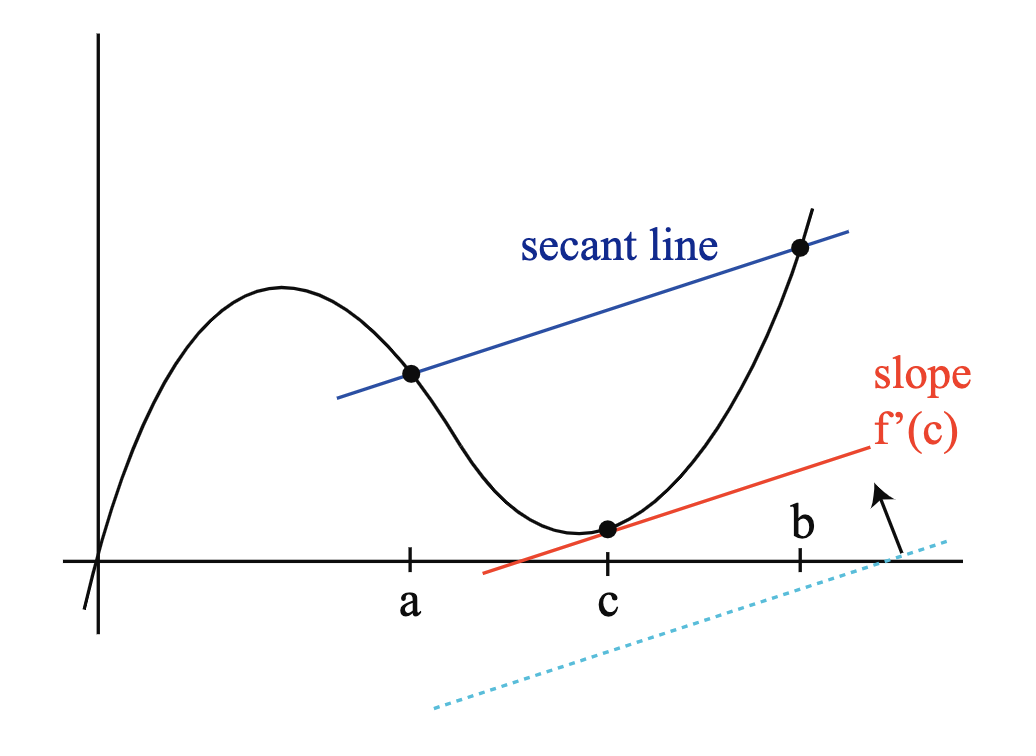
\includegraphics[scale=0.7]{./images/lecture_9_figure_1.png}
	\caption{Illustration of the Mean Value Theorem}
\end{figure}

\textbf{Geometric Proof: } Take dotted lines parallel to the secant line and shift them up until it touches the graph.
Alternatively one may have to start from above the graph and move it down until it touches.

If the function $f$ isn't differentiable, this approach goes wrong.
For instance, it breaks down for function $f(x) = |x|$. 
The dotted line always touch the graph at $x=0$, no matter what the slope is, and $f'(0)$ is undefined.

\begin{figure}[ht!]
	\centering
	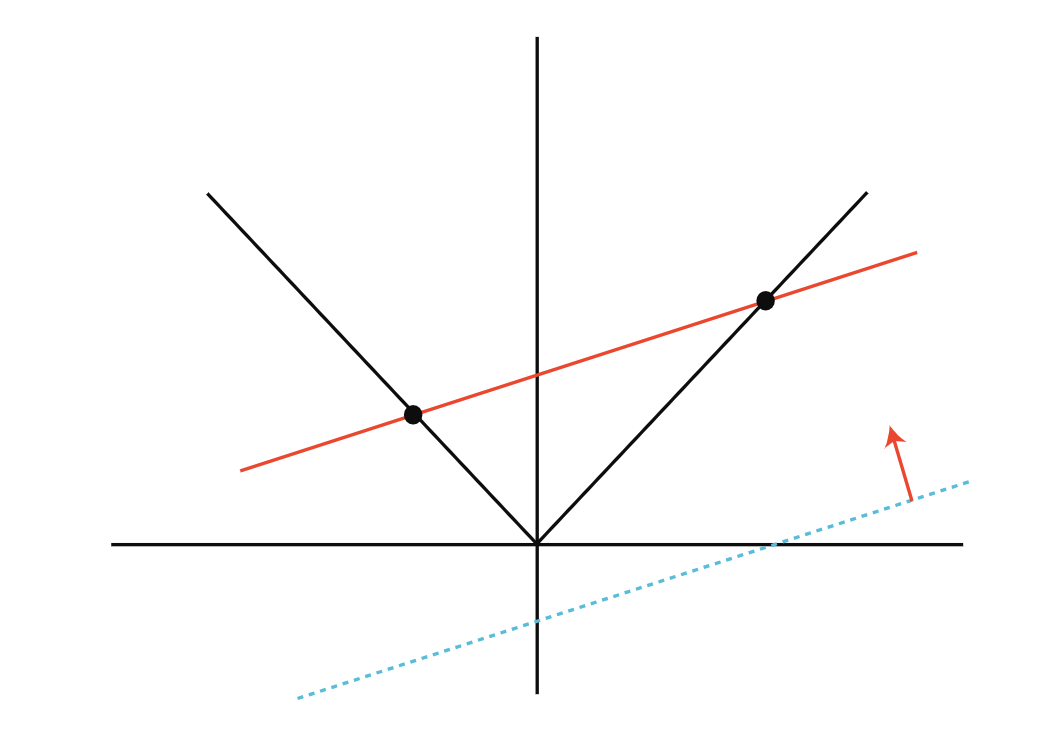
\includegraphics[scale=0.7]{./images/lecture_9_figure_2.png}
	\caption{Graph of $y = |x|$, with secant line. (MVT goes wrong.)}
\end{figure}

\section{Versions of Mean Value Theorem}

There is a second way of writing MVT:
\begin{align*}
    f(b) - f(a) & = f'(c)(b-a) \\ 
    f(b) & = f(a) + f'(c)(b-a) \quad \text{ (for some $c, a < c < b$)}
\end{align*}
There is also a third way of writing MVT: change the name of b to x.
$$ \boxed{ f(x) = f(a) + f'(c)(x-a) \quad \text{ for some } c, a < c < x } $$


\section{Uses of Mean Value Theorem}

\begin{enumerate}
    \item If $f' > 0$, then $f$ is increasing.
    \item If $f' < 0$, then $f$ is decreasing.
    \item If $f' = 0$ all $x$, then $f$ is constant.
\end{enumerate}